\chapter{Zaplecze technologiczne - wykorzystane biblioteki}
\label{chapter:libs}

\section{Spring Framework}
	\textbf{Spring} jest szkieletem tworzenie aplikacji w języku Java dla platformy Java (Standard Edition oraz Enterprise Edition). Jego największą zaletą jest lekkość szablonu, który nie wymusza konkretnego stylu programowania czy też zewnętrznych bibliotek do użycia, jednocześnie dając możliwość integracji praktycznie dowolnej biblioteki zewnętrznej. Dobrym przykładem jest mnogość opcji do wyboru w przypadku pisania warstwy widoku aplikacji webowej. Spring oferuje wsparcia czystego JSP (ze wsparciem tagów JSTL) jednocześnie dając możliwość użycia takich bibliotek jak Velocity, FreeMarker, XSLT czy Apache Tiles. 
	Kolejnym ważnym punktem wartym wspomnienia, a będącym fundamentem na którym oparta jest aplikacja będąca jednym z podmiotów pracy inżynierskiej jest budowa framework'a. Poszczególne moduły zostały zaprojektowane tak, że mogą działać samodzielnie, dzięki czemu programista może wybierać je dowolnie, nie będąc zmuszonym do wyboru innych. Wykorzystane zostały więc następujące moduły:
	
	\begin{figure}[H]
		\centering
		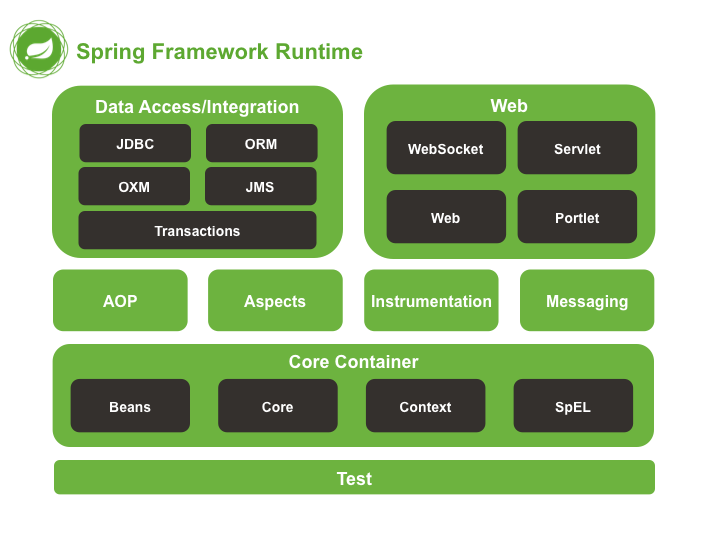
\includegraphics[width=0.95\textwidth]{images/spring-overview}
		\caption[Kontener Spring]{
			Kontener Spring wraz z modułami\\ 
			źródło: \cite{spring_documentation_reference}
		}
		\label{c3:information_level_figure}
	\end{figure}
	
	\subsection{Wykorzystanie możliwości Spring'a}
		Wykorzystanie szkieletu aplikacji \textbf{Spring} stanowi główną część praktycznej w rozumieniu użytych bibliotek oraz 
		frameworków. Głównym powodem była mnogość opcji oferowanych przez sam framework oraz ogromna ilość technologii z którymi
		można było go zintegrować. Dzięki gotowemu wsparciu dla konwersji danych oraz ich walidacji udało się zaoszczędzić
		dużą ilość czasu.
		
	\subsection{Użyte moduły Spring'a}
	
	% modules descriptions goes here 
	\paragraph{Spring Core}
		Zgodnie z nazwą - \textbf{Spring Core} - jest to moduł podrzędny Spring' oraz jednocześnie jego główna część. Dostarcza funkcjonalności \textit{IoC} oraz \textit{Dependency Injection}. \todo[inline]{Describe IoC and DI}
		Zawarte w nim implementacje wzorca fabryki, pozwalają na transparentne, z punktu widzenie programisty, tworzenie oraz korzystanie z \textbf{singletonów} - domyślny cykl życia tworzonych w kontenerze obiektów. 
		\textit{Context} stanowi rozszerzenie powyższego modułu o możliwości definiowania kontekstu aplikacji. Kontekst jest w tym wypadku tak naprawdę tym, co określa i zbiera informację o tym co w danym momencie w aplikacji działa. Niemniej możliwe jest także tworzenie, a dokładniej pobieranie nowych obiektów z kontekstu, gdzie w przypadku kiedy one jeszcze nie istnieją - tworzenie ich.
		\textit{SpEL} jest językiem wyrażeń pozwalających na dostęp cy też modyfikację danych poprzez napisania wyrażenie \textbf{SpEL}, które zostanie następnie użyte, aby określić właściwy ciąg wykonania instrukcji zawartych w samym wyrażeniu. Jest to jednocześnie rozszerzenie \textbf{Unified Expression Language}, do którego dodano elementy właściwe dla framework'a Spring. Dzięki czemu programista może w łatwy sposób napisać wyrażenie, którego celem jest wywołanie pewnej metody z serwisu\footnote{Serwis, czyli klasa opatrzona adnotacją \texttt{@Service} } istniejącego w kontekście. \cite{unified_el}\cite{spring_documentation_reference}. Ponadto \textit{SpEL} jest zintegrowany z modułem \textbf{Spring}, którego głównym zadaniem jest konwersja z jednego typu na drugi. Dzięki temu nie ma potrzeby dokonywania jawnego rzutowania z jednego typu na drugi. Wystarczy jedynie zadeklarować konwerter lub użyć jednego z już istniejących.
		Aplikacja demonstracyjna używa języka wyrażeń na dwa sposoby. Pierwszym z nich jest jawne użycie, najczęściej występujące w warstwie widoku na stronach używających komponentów takich jak: \textbf{tabele} czy \textbf{strony obiektów}. Drugim jest niejawne użycie w definicjach \textbf{Web Flow}. Definicja konkretnego przepływu napisana jest w formacie XML. Niemniej nie byłaby ona użyteczna, gdyby nie zawierała elementów pozwalających na reagowania na pewne zdarzenie poprzez wywołania obiektów logiki biznesowej. Słowem kluczowym są tutaj \textbf{wywołania} pisane właśnie w \textbf{SpEL}. 	
		
	\paragraph{Spring MVC}
	\label{app:spring_mvc}
	\textbf{MVC}\footnote{\textbf{M}odel-\textbf{V}iew-\textbf{C}ontroller} jest wzorcem programistycznym 
	właściwym dla implementowania warstwy interfejsu użytkownika, gdzie nacisk położony 
	jest na ścisłe odseparowanie warstw \textbf{widoku},\textbf{dostępu do danych} oraz 
	\textbf{logiki biznesowej}. \textbf{Spring MVC} jest zorganizowany wokół 
	centralnego servletu \texttt{DispatcherServlet} oraz klas z adnotacjami 
	\texttt{@Controller} lub \texttt{@RestController} - \textbf{kontrolerów}. 
	Adnotacje są implementacją konfigurowalnego mapowania adresów. Korzystając 
	z takiego podejścia, programista nie jest zmuszony do definiowania kilku, 
	bądź kilkunastu oddzielnych servletów, z których każdy odpowiada innemu 
	przypadkowi użycia\footnote{\textbf{Przypadek użycia} (ang. usecase) jest sposobem 
	opisu wymagań aplikacji na poziomie interakcji między użytkownikiem końcowym 
	(aktorem), a systemem} lub pisania własnego silnika, który pozwalał by na generyczne 
	i automatyczne wywołania konkretnych metod lub klas w zależności od podanego adresu lub jego części. 
	Oprócz kontrolerów, \texttt{DispatcherServlet} wspiera także klasy, których 
	zadaniem jest implementacja walidacji obiektów używanych w formularzach. 
	Same obiekty nie podlegają żadnym konkretnym regułom wymuszonym przez framework. 
	Są to tak zwane \textbf{POJO}. Spring jest odpowiedzialny za ewentualne walidacja, transformacje (z/do XML'a lub JSON'a) lub konwersje. 
	Ostatecznie programista nie jest zmuszony do wykorzystanie konkretnej warstwy 
	widoku, ponieważ \textbf{Spring MVC} daje możliwości korzystania z wielu 
	różnych widoków w wielu różnych kontekstach. Zależnie więc od przypadku użycia widok 
	może być rozumiany jako zwykły plik JSP, jako część lub konkretny widok w technologii 
	\textbf{Apache Tiles}, a nawet plik PDF. Ponadto istnieje wsparcie dla widoków 
	ładowanych przez \textbf{Ajax}, co bezpośrednio przekłada się na zoptymalizowanie częściowe ładowania stron.

	\paragraph{Spring Data - Spring Data JPA}
	\label{app:spring_data}
	\textbf{Spring Data} jest praktycznym rozwiązaniem problemu związanego z implementacją warstwy dostępu do danych. 
	Ów problem odnosi się do pisania szablonowego kodu, którego głównym zadaniem jest wykonanie operacji określanych 
	skrótem \textbf{CRUD}\footnote{CRUD - \textit{Create}-\textit{Read}-\textit{Update}-\textit{Delete} - zbiór czterech 
	podstawowych funkcji w aplikacji korzystających z pamięci trwałej jako nośnika przechowywania danych, które 
	umożliwiają zarządzanie nimi.}. Przy jednoczesnym zapewnieniu prostoty użytkowania, bardzo wysokim poziomie 
	abstrakcji jest to biblioteka dzięki której ilość właściwego kodu, a przez to jego efektywność, realizującego 
	specyficzne wymagania danej aplikacji jest maksymalnie niska. Warto w tym miejscu zwrócić uwagę na generyczne 
	API, które przekłada się na wspomniany poziom abstrakcji, dzięki któremu możliwe jest korzystania z praktycznie
	dowolnego źródła danych przez zunifikowany interfejs. Nie ważne staje się, czy dane przechowywane są w bazie 
	danych \textbf{MySQL} lub \textbf{Oracle}, czy też w bazach nierelacyjnych jako \textbf{Mongo}. 
	Dzięki temu otrzymany kod jest wysoce przenośny, a zmiana źródła danych wiążę się jedynie z poprawkami 
	w definicji modelu danych. Ponadto elementy takie ujednolicona hierarchia wyjątków, rozszerzalność 
	stanowią wspólnie o sile \textbf{Spring Data}.
	
	\label{tech:spring_data_jpa}
	\textbf{Spring Data JPA} jest pod modułem \textbf{Spring Data}, które zawiera klasy oraz interfejsy szczególnie użytecznie jeśli
	źródło danych aplikacji jest relacyjną bazą danych jak na przykład MySQL. Jednym z tych elementów są repozytoria.
	Repozytorium jest niczym innym jak obiektem w naszej aplikacji dzięki któremu uzyskujemy faktyczny dostęp do danych i możemy
	nimi zarządzać dzięki wspomnianym operacjom CRUD. Co ważniejsze pojęcie to jest znacznie szersze niż mogłoby
	się wydawać, zwłaszcza w kontekście operacji wyszukiwania. Poniższy przykład kodu pokazuje jedynie klasę \textbf{JpaRepository}. 
	Istniejące tam deklaracje metod są jedynie rozszerzeniem tych zdefiniowanych w dwóch interfejsach, kolejne z siebie dziedziczących, z
	których \textbf{JPA Repository} rozszerza. Niemniej widać, że nawet na wyższym poziomie programiści \textbf{Spring Data} zadbali o bardzo
	wiele możliwych przypadków użycia, co przekłada się na końcową produktywność programisty. 
	\begin{code}
		\inputminted[
			lineos=true,
			fontfamily=monospace,
			obeytabs=true,
			samepage=true,
			fontsize=\scriptsize
		]{java}{codeSamples/jpa_repo.java}
		\label{tech:jpa_repo}
		\caption[\textbf{JpaRepository}]{\textbf{JpaRepository} interfejs dla operacji bazodanowych na relacyjnej bazie danych w \textbf{Spring Data}}.
	\end{code}
	Ponadto programista nie jest zmuszony do implementacji takiego interfejsu, a jedynym jakie zadanie jest stworzenie własnego interfejsu, który będzie
	posiadał typy generyczne zgodne z jego przeznaczeniem. Klasa zostanie zaimplementowana podczas działania programu poprzez proxy. 
	Repozytoria posiadają także inną bardzo interesującą cechą - automatyczne mapowaniem metod na kwerendy. Jest to pewna alternatywa dla znanych ze standardu
	\textbf{JPA} nazywanych kwerend (named queries). Definicja zapytania SQL pobierana jest z nazwy metody, co oczywiścia wymusza pewną konwencję nazewnictwa. 
	Niemniej jest to koncepcja ciekawa i idealnie nadaje się do tworzenia zapytań odnoszących się do 1 lub 2 atrybutów danego obiektu. Wywołanie jest silnie
	typizowane dlatego programista ma pewność, że obiekt typu, który go interesuje zostanie zwrócony. Dla bardziej skomplikowanych kwerend istnieje
	możliwość zadeklarowanie metody i oznaczenia ją adnotacją \textit{\@{}Query} z kodem JPQL\cite{jpql} dla interesującego nasz przypadku\cite{spring_data}.
	
	Jak widać \textbf{Spring Data} jest dobrze zaprojektowanym modułem, dzięki któremu programista może oszczędzić dużo czasu, którego potrzebowałby 
	na przygotowanie całej warstwy abstrakcji potrzebnej do wykonywania wszelakiego rodzaju operacji, bez skupienia się na źródle swojego problemu - logice
	aplikacji. 

	\paragraph{Spring Security}	
	W momencie pisania aplikacji w technologii \textbf{Java EE}\footnote{Java Enterprise Editition} nie można zapomnieć o problemie nieautoryzowanego dostępu do strony lub do niektórych jej części. Sposób uzyskania takiej funkcjonalności jest zależny od kontenera w którym działamy. Inaczej to zagadnienie rozwiązywane jest w przypadku \textbf{Apache Tomcat},a inaczej w przypadku \textbf{JBoss}. Oba z nich są serwerami aplikacji Javy, niemniej tak samo jak identyczny jest cel ich istnienia, tak samo różna jest implementacja kwestii autoryzacji. Dzięki \textbf{Spring Security} programista może korzystać z niezależnego od kontenera wysoce konfigurowalnego mechanizmu kontroli dostępu do zasobów. W tym miejscu warto nadmienić, że moduł można dostosować do korzystanie weryfikacji użytkowników zarówno z wykorzystaniem bazy danych, stałej listy. Ponadto niewielkim nakładem pracy można dodać mechanizm kontroli znany pod nazwą \textbf{Access Control List}. Jest to koncepcja gdzie prawa dostępu (zarówno zapisu, odczytu czy tez modyfikacji) związane są z konkretnym typem obiektu. Wszystkie wyżej wymienione cechy czynią \textbf{Spring Security} doskonałym wyborem do ochrony wrażliwych elementów aplikacji internetowej. 

	\paragraph{Spring HATEOAS}\cite{spring_hateos}
	Jest to praktyczna implementacja paradygmatu znanego jako \textbf{HATEOAS - Hypermedia as the Engine of Application State} dla aplikacji wykorzystujących inny ze znanych koncepcji - \textbf{REST}. W przypadku \textbf{HATEOAS} duży procent funkcjonalności aplikacji jest oferowany w postaci hiperłączy powiązanych z obiektami. To co wyróżnia to podejście jest fakt, że klienci nie muszą znać funkcjonalności do momentu kiedy jest ona im prezentowana na stronie internetowej. Jest to możliwe ponieważ poza łączami przekierowującymi lub uruchamiającymi konkretne funkcje z serwera przekazywana są etykiety, które w czytelny sposób sygnalizują efekt akcji. 
	W kontekście \textbf{Spring HATEOAS} należy wspomnieć, że rozwiązane jest zintegrowane z \textbf{Spring Data} i korzysta z tzw. repozytoriów danych jako źródła przez które udostępnia akcje - łącza dla każdego z obiektów. Przykładowa odpowiedź w rozumieniu tego paradygmatu mogłaby wyglądać następująco:
	\begin{code}
		\begin{minted}[fontfamily=courier,obeytabs=true,samepage=true,fontsize=\small]{json}
{
    "name"	   	: "John",
    "lastname"	: "Doe",
    "links"	   	: [
        {
            "rel" : "self",
            "href": "http://localhost/customer/1"
        },
        {
            "rel" : "parent",
            "href": "http://localhost/customer/1/parent"
        }
    ]
}
		\end{minted}
		\label{app:spring_hetoas_response_example}
		\caption[Spring HATEOAS - Przykładowa odpowiedź]{Przykładowa odpowiedź serwera na akcję w rozumieniu paradygmatu HATEOAS}
	\end{code}

	\paragraph{Spring Web Flow}	
	\begin{quotation}
		``Przemieszczenia się kogoś, czegoś, przekazywanie, obieg czegoś.''\cite{polish_dictionary}
	\end{quotation}
	\textbf{SWF}\footnote{Skrót od Spring Web Flow} jest szczególnie użyteczne gdy aplikacja wymaga powtarzalności tych samych kroków
	w więcej niż jednym kontekście. Czasami taka sekwencja operacji jest częścią większego komponentu co desygnuje je do wyodrębnienia
	ich jako re używalnego komponentu. Najlepszym przykładem użycia są w tym wypadku różnego rodzaju formularze służące do rejestracji
	użytkowników czy tez kreatory nowych obiektów, gdzie umieszczenie wszystkich wymaganych pól na jednej stronie mogłoby zaciemnić obraz
	i uniemożliwić użytkownikowi zrozumienie działania. 
	Z racji, ze \textbf{SWF} jest modułem Spring, jest on w pełni zintegrowany z platformę \textbf{Spring MVC}\ref{app:spring_mvc} oraz
	silnikiem walidacji i konwersji, dzięki czemu programista nie jest zmuszony do tworzenia własnych rozwiązań tego typu. 
	
	\textbf{Flow}\cite{spring_swf_reference} - jest centralnym obiektem modułu, w którym definiowane są kolejne kroki przepływu. Dzięki
	deklaratywnemu językowi XML definicje są czytelne, a możliwości których dostarcza \textbf{SWF} pozwala na kreowania sekwencji
	w dowolny sposób, łączenie kroków z modelem danych, korzystania z podstawowych jak i zaawansowanych mechanizmów implementacji
	akcji. Akcje zawierają właściwą logikę biznesową dla konkretnej fazy działania, w której możemy definiowania operacje takie
	jak pobranie danych wejściowych czy też obsługa wyjątków. 
	
	\begin{code}
		\inputminted[
			lineos=true,
			firstline=47,
			lastline=55,
			fontfamily=monospace,
			obeytabs=true,
			samepage=true,
			fontsize=\scriptsize
		]{xml}{../SpringAtom/src/main/webapp/ui/wizard/NewReportWizard/flow.xml}
		% src file used
		\label{app:swf_view_state}
		\caption[Definicja kroku Spring Web Flow]{\textit{../NewReportWizard/flow.xml} - deklaratywna deklaracja stanu - kroku 
		dla przepływu w rozumieniu \textbf{Spring Web Flow}}.
	\end{code}
	Przykład \ref{app:swf_view_state} pokazuje kod XML, który definiuje jeden z kroków - stanów. Powyższy przykład korzysta z klasy
	\begin{code}org.springframework.webflow.action.FormAction\end{code}. Przykładowo metoda \begin{code}setupForm\end{code} może
	służyć między innymi do wprowadzenia danych wejściowych do kontekstu przepływu.
	\begin{code}
		\inputminted[
			lineos=true,
			firstline=69,
			lastline=76,
			fontfamily=monospace,
			obeytabs=true,
			samepage=true,
			fontsize=\scriptsize
		]{java}{../SpringAtom/src/main/java/org/agatom/springatom/web/flows/wizards/wizard/rbuilder/PickEntityFormAction.java}
		% src file used
		\label{app:swf_setupForm}
		\caption[Metoda \textit{setupForm} dla \textbf{Spring Web Flow}]{\textit{PickEntityFormAction\#{}setupForm} - metoda
		\textit{setupForm} wykorzystywana w definicji kroku \ref{app:swf_view_state} do umieszczenia danych w kontekście
		przepływu.}
	\end{code}

	\paragraph{Spring Test}
	Testowanie w aplikacjach, zarówno biznesowych, ale także i tych których zasięg ograniczony jest do lokalnych odbiorców, jest
	krytycznym punktem każdego programu. Test, w rozumieniu języków programowania, należy rozumieć jako kod, a dokładniej pojedynczą
	metodą lub ich zbiór, które wywołują inne metody i weryfikują poprawność zwróconych danych pod kątem zadanych danych wejściowych.
	Jeśli wyniki różnią się od oczekiwanych oznacza to, że test nie wykonał się poprawny.
	Dobry test jednostkowy charakteryzuje się:
	\begin{itemize}
		\item powinien być zautomatyzowany i wykonywalny wielokrotnie,
		\item powinien być łatwy w implementacji,
		\item raz napisany, powinien być wykorzystywany,
		\item nie powinien pozostawiać w testowanym systemie pozostałości swojego działania,
		\item powinien wykonywać się w miarę szybko.
	\end{itemize} \cite{the_art_of_unit_testing}.
	
	\textbf{Spring Test} zostało stworzone aby uprościć proces testowania kodu aplikacji. Oferuje wsparcia dla wielu różnych
	framework'ów przeznaczonych do testów jednostkowych takich jak \textbf{JUnit} lub \textbf{TestNG}, czy też bibliotekami, których
	celem jest dostarczanie rozwiązań umożliwiających tak zwane \textit{mockowanie}\footnote{Mock - obiekt, który symuluje działanie
	prawdziwego obiektu. Tworzony jest aby kontrolować przebieg testu w symulowanych warunkach}. 
	
	Z racji tego, że omawiany tutaj moduł jest częścią \textbf{Spring Framework} należy wspomnieć o pełnej integracji z poszczególnymi
	funkcjami. Elementy takie jak wsparcie dla \textit{Dependency Injection}, pozwalają pisać testy dla obiektów działających w
	środowisku \textbf{MVC} czy też serwisów bazodanowych\footnote{Serwis bazodanowy - Klasa opatrzona adnotacją \textit{\@{}Service}.
	Różni się ona od klas obsługujących operacje \textbf{CRUD} z uwagi na to, że ich głównym zadaniem jest dostarczanie funkcjonalności
	logiki biznesowej}. 
	
	% modules descriptions goes here
	
\section{JPA - Java Persistance API}\label{tech:jpa}
	\textbf{JPA - Java Persistance API} jest standardem określającym reguły opisu mapowania obiektowo-relacyjnego dla języka \textbf{Java}. W aplikacji demonstracyjnej \textbf{JPA} została zastosowana do: opisania wszystkich obiektów należących do modelu danych na poziomie nazw tabel, nazw oraz ograniczeń kolumn oraz wzajemnych powiązań między różnymi obiektami, czyli innymi słowy relacji klucz główny-klucz obcy na poziomie tabel w bazie danych. Użycie standardu jako sposobu specyfikacji modelu danych, zostało podyktowane wykorzystaniem tego samego standardu przez inne biblioteki, a w konsekwencji moduły aplikacji. 
	
\section{Hibernate - Object Relational Mapping}\label{tech:hibernate}
	Wykorzystanie \textbf{Hibernate} w aplikacji jest w głównej mierze transparentne. Dzięki wykorzystaniu \textbf{Spring Data (\ref{app:spring_data})}
	silnik ORM może zostać całkowicie wyłączony z operacji bazodanowych. Niemniej jego cecha jako wykonawcy mapowania obiektowo relacyjnego jest wciąż wykorzystywana. W swojej najnowszej wersji \textbf{Hibernate}, pomijając część wyjątkowych sytuacji specyficznych dla siebie, opiera się o standard \textbf{JPA}(\ref{app:jpa}). Takie podejście pozwala ponownie na zaprojektowanie modelu danych którego przenośność jest wysoka, a migracja do innego szkieletu aplikacji ORM ogranicza się do wybrania takiego, który obsługiwałby standard. 

\section{c3pO}
	\textbf{c3p0} jest łatwą do użycia biblioteką zaprojektowaną dla \textbf{Java}, której głównym zadaniem jest realizacja postulatów zdefiniowanych
	przez specyfikacją \textbf{jdbc3}. Dzięki powyższej bibliotece można w łatwy sposób zdefiniować \emph{n} - połączeń z bazą danych, gdzie kolejne
	z nich będą wykorzystywane jeśli kolejka żądań do innych będzie już pełna. Także elementy takie jak zarządzania zajętymi zasobami, ich zwalnianie są obsługiwane przez \textbf{c3p0}. Dzięki wsparciu dla szkieletu aplikacji \textbf{Spring} konfiguracja okazuje się trywialna i polega na zadeklarowaniu
	odpowiedniego \textbf{bean'a} w konfiguracji XML lub Java \cite{c3p0}.
	
\section{QueryDSL}
	\textbf{QueryDSL} jest projektem \textit{OpenSource}, którego użyciu wynika z korzystania z \textbf{Spring Data JPA (\ref{app:spring_data})}. Jego główną zaletą jest możliwość interakcji z bazą danych na wysokim poziomie abstrakcji, gdzie nie jest znane, ponieważ nie ma takiej potrzeby, z jakiego silnika bazy danych korzysta aplikacja. Ponadto, w porównaniu z API Hibernate, \textbf{QueryDSL} pozwala na konstruowania silnie typizowanych zapytań lub bardziej ogólnie kwerend \textbf{HQL}\footnote{Hibernate Query Language - język kwerend SQL zorientowany obiektowo} konstruowanych w oparciu o typ znakowy \textsc{java.lang.String}. Dzięki temu programista nie jest zmuszony do rzutowania oraz wcześniejszego sprawdzania, czy obiekt który chce uzyskać odpowiada jego wymaganiom.
	Podczas pracy z \textbf{QueryDSL} najistotniejszym elementem jest model, który generowany jest z modelu danych podczas kompilacji przez \textbf{ATP}.
	Ważną cechą meta modelu jest jego niezależność od faktycznie używanego silnika danych, a najważniejszą zaletą jest to, że uzyskanym efektem są
	zwykłe klasy Java, dzięki czemu programista ma możliwość konstruowania kwerend ze wsparciem uzupełniania składni. 
	
\section{Ehcache}
	\textbf{Ehcache} jest biblioteką \textit{OpenSource} dostarczającą funkcjonalność pamięci podręcznej dla aplikacja Java oraz Java Enterprise. 
	Główną zaletą posiadania takiego rozwiązania jest odciążanie bazy danych, ponieważ 	część zapytań oraz ich wyników zapisana jest w pamięci lub w systemie plików. 
	Użyteczność tej biblioteki potwierdza zasada znana, jako \textbf{zasada Pareto}, czyli stosunku 80:20. 
	Jeśli weźmiemy pod uwagę 20\% obiektów (np. rekordów z bazy danych),które używane są przez 80\% czasu działania aplikacji to 
	używając pamięci podręcznych możemy poprawić wydajność aplikacji o koszt uzyskania 20\% obiektów.
	
	W ogólnym zarysie idea działania pamięci podręcznej opiera się na tablicy asocjacyjnej, gdzie każdemu z unikatowych kluczy odpowiada pewna wartość.
	Podczas umieszczanie obiektu do pamięci obliczana jest unikatowa wartość klucza, po której owa wartość będzie identyfikowana. Samą pamięć można opisać jako,
	miejsce gdzie umieszcza się obiekty, które duplikują inne, ale do których dostęp jest bardziej długotrwały i wymaga dostępu np. do bazy danych, lub do obiektów,
	które są wynikami pewnych obliczeń. Podczas próby pobrania elementu z cache'u można mówić o pojęciu \textbf{hit} - element dla danego klucza zostaje znaleziony
	oraz o pojęciu \textbf{miss}, kiedy element o danym kluczu nie istnieje w pamięci podręcznej.\cite{ehcache_documentation_ref}
	
	\subsection{Warstwa abstrakcji Spring dla cache'owania obiektów}
		W aplikacji demonstracyjnej \textbf{Ehcache} nie jest używany bezpośrednio, pomijając tworzenie domyślnych cache'ów. Cała funkcjonalność odnosząca się do ewentualnego pobierania, umieszczania oraz usuwania obiektów z odpowiadających im pamięci podręcznych realizowana jest na poziomie adnotacji:
		\begin{center}
			\begin{longtable}{| p{3cm} | p{13cm} |}
				\caption[Adnotacje Spring opisujące poziom abstrakcji cache]{
					Adnotacje Spring opisujące poziom abstrakcji cache				
				}\tabularnewline	
				
				\hline
					\multicolumn{1}{|c|}{\textbf{Adnotacja}} &
					\multicolumn{1}{|c|}{\textbf{Funkcjonalność}} \tabularnewline
				\hline
				\endfirsthead
				
				\multicolumn{2}{c}
				{{\bfseries \tablename\ \thetable{} -- kontynuacja...}} \tabularnewline
				\hline
					\multicolumn{1}{|c|}{\textbf{Adnotacja}} &
					\multicolumn{1}{|c|}{\textbf{Funkcjonalność}} \tabularnewline
				\hline
				\endhead
					
				\hline
					\multicolumn{2}{|r|}{{Następna strona...}} \tabularnewline \hline
				\endfoot

				\hline \hline
				\endlastfoot	
				
				\emph{Cacheable}\footnote{\url{http://docs.spring.io/spring/docs/4.0.0.RELEASE/javadoc-api/org/springframework/cache/annotation/Cacheable.html}} &
				Adnotacja odnosi się do konkretnej metody lub całej klasy (w tym wypadku 
				wszystkich zdefiniowanych w niej metod) i wskazuje, że ich argumenty mają być użyte 
				od obliczenie klucza a wartości zwracane przez te metody będą odpowiadać wartościom klucza. 
				Faktyczne umieszczenie obiektu w pamięci podręcznej może być pominięte
				jeśli istnieje on już w cache'u \tabularnewline
				\hline
				\emph{CachePut}\footnote{\url{http://docs.spring.io/spring/docs/4.0.0.RELEASE/javadoc-api/org/springframework/cache/annotation/CachePut.html}} &
				Działa podobnie jak powyższa adnotacja z tą różnicę, że każdorazowe 
				wywołania metody opatrzonej tą adnotacją powoduje umieszczenie obiektu
				w pamięci podręcznej \tabularnewline
				\hline
				\emph{CacheEvict}\footnote{\url{http://docs.spring.io/spring/docs/4.0.0.RELEASE/javadoc-api/org/springframework/cache/annotation/CacheEvict.html}} &
				W przeciwieństwie to \emph{CachePut} oraz \emph{Cachable} wskazuje, 
				że wywołania metody nią opatrzonej spowoduje usunięcie z pamięci podręcznej obiektu
				o danym kluczu
			\end{longtable}
			\label{app:ehcache:spring_caches}
		\end{center}
		
\section{Apache Tiles}\label{tech:tiles}
	\textbf{Apache Tiles} to biblioteka umożliwiająca dekompozycję widoku aplikacji na wiele niezwiązanych ze sobą bezpośrednio elementów - płytek \footnote{Z angielskiego tiles może oznaczać płytkę, w kontekście technologii ApacheTiles należy rozumieć to wyrażenie, jako element, który można wykorzystać w dowolnym szablon}. Płytki można potem dowolnie łączyć w konkretne widoki definiując je na poziomie plików XML. Główną zaletą korzystanie z podejścia ze wzorca kompozycji jest wyeliminowanie powielania się elementów stron i zastąpienie ich szablonami gotowymi do użycia w dowolnym miejscu. Dodatkową zaletą użycia tej biblioteki było gotowe wsparcie dla modułu Spring’a – Spring Webflow\ref{app:techonlog_spring_webflow}, gdzie jedną z preferowanych technologii widoku jest właśnie Apache Tiles, a także możliwość prostszego wsparcia dla \textbf{partial rendering}\footnote{Partial rendering należy rozumieć, jako usunięcie konieczności przeładowania całej strony WEB, a jedynie jej konkretnej części.} stron, gdzie podczas przechodzenia do innego adresu w rzeczywistości zamiast ładować całość strony wraz ze wszystkimi plikami \textit{CSS} oraz \textit{JavaScript}, ładuje się jedynie konkretną zawartość.
	
\section{Jasper Reports/Dynamic Jasper}\label{tech:jasperReports}
	\textbf{Jasper Reports} to kompleksowe rozwiązanie dla języka \textbf{Java} wspierające tworzenie oraz generowanie reportów
	biznesowych dla wielu różnorodnych formatów wyjściowych: \textbf{PDF}, \textbf{XLS}, \textbf{CSV} i wielu innych. Jego główną
	zaletą jest pojedynczy format przechowywania raportu oraz mnogość formatów reprezentacji, a także ogromna ilość
	narzędzi oraz bibliotek wspierających tworzenie, modyfikacje raportów. 

	Z drugiej strony wiele tych narzędzi jest aplikacjami uruchamianymi na komputerach użytkowników, a nie
	zaprojektowanych do wykorzystania w środowisku aplikacji WEB. Z tego powodu właściwą biblioteką, która została
	użyta celem utworzenia raportu jest \textbf{Dynamic Jasper}. Działając po stronie serwera oraz bazując
	na danych wejściowych uzyskanych od użytkownika pozwala na kompilację do pliku \textit{*.jasper}. 
	Możliwe jest ustalenie takich właściwości jak nagłówki, styl, ilość kolumn oraz typ danych w nich przechowywanych.

\section{Dandelion Datatables}\label{tech:dandelion}
	\textbf{Dandelion-Datatables} jest biblioteką zaprojektowaną dla języka \textbf{Java}, której zadaniem jest wsparcie
	dla tworzenie tabel korzystając z użyciem tagów JSP. Instrukcje dostarczane tą drogą uruchamiają proces generowania
	kodu JavaScript dla wtyczki \textbf{jQuery} - \textbf{DataTables}. Nie ma konieczności bezpośredniego
	pisania kodu JS co pozwala na budowania responsywnych tabel bez znajomości języka JavaScript. 
	\textbf{Dandelion Datables} pozwala na bezproblemowe sortowanie, filtrowanie oraz eksportowanie danych. 